

Dados dos conjuntos $A$ y $B$, el conjunto intersección de estos, que se
designará como $A \cap B$ y se leerá ``$A$ intersección $B$'', es el
conjunto de los elementos comunes de ambos conjuntos. Es decir,

\[ A \cap B = \{x \st x \in A \ \text{y} \ x \in B\} \]

\noindent o, con notación más propia de la lógica,

\[ A \cap B = \{x \st (x \in A) \land (x \in B)\} \]

En particular, si $A$ y $B$ son subconjuntos del conjunto $U$ y están
definidos por comprensión, es decir,

\[ A = \{x \in U \st P_x\}, \quad B = \{x \in U \st Q_x\} \]

\noindent entonces

\[ A \cap B = \{x \in U \st P_x \land Q_x\} \]

\begin{example}
  Si

  \begin{align*}
    A = \{a, b, c, d, e, h\} \\
    B = \{g, a, b, d, h, i, j\} \\
  \end{align*}

  \noindent entonces

  \[ A \cap B = \{a, b, d, h\} \]
\end{example}

En la figura~\ref{fig:venn-union-interseccion}, se ha representado un
diagrama de Venn de los conjuntos $A$ y $B$ donde se ha sombreado el
conjunto $A \cup B$ intensificando el sombreado de $A \cap B$. En un
diagrama de Venn, se ve muy fácilmente que

\[ A \cap B \subseteq A \cup B \]

\noindent aunque también se puede demostrar de otras formas.

% TODO Completar la parte interna, que no se ve bien en el PDF.

\begin{figure}
  \centering
  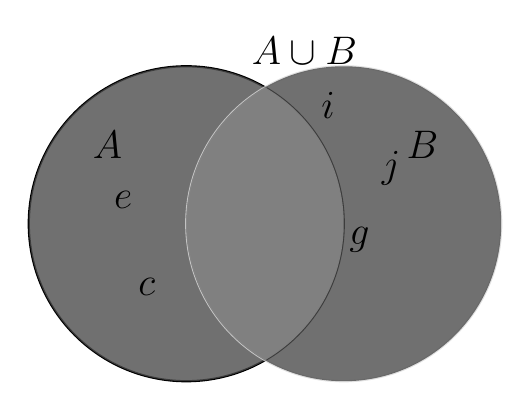
\begin{tikzpicture}
    % Conjunto A
    \draw[thick] (0,0) circle (2);
    \fill[gray!140, opacity=0.8] (0,0) circle (2);
    \node at (-1, 1) {\Large $A$};

    % Conjunto B
    \draw[thick, gray!30, opacity=0.8] (2,0) circle (2);
    \fill[gray!140, opacity=0.8] (2,0) circle (2);
    \node at (3, 1) {\Large $B$};

    % Región de intersección (A ∩ B)
    \begin{scope}
        \clip (0,0) circle (2);
        \fill[gray!90, opacity=0.8] (2,0) circle (2);
    \end{scope}

    % Etiqueta de la unión
    \node at (1.5, 2.2) {\Large $A \cup B$};

    % Etiquetas de elementos
    \node at (-0.8, 0.3) {\Large $e$};
    \node at (-0.5, -0.8) {\Large $c$};
    \node at (2.6, 0.7) {\Large $j$};
    \node at (2.2, -0.2) {\Large $g$};
    \node at (1.8, 1.5) {\Large $i$};

  \end{tikzpicture}
  \caption{Diagrama de Venn de $A \cup B$ y $A \cap B$}%
  \label{fig:venn-union-interseccion}
\end{figure}

\begin{example}
  Dados los conjuntos

  \begin{align*}
    C &= \{x \in \nset \st x \ \text{es múltiplo de} \ 2\} \\
    D &= \{x \in \nset \st x \ \text{es múltiplo de} \ 3\} \\
  \end{align*}

  \noindent entonces

  \[ C \cap D = \{x \in \nset \st x \ \text{es múltiplo de} \ 2 \ \text{y
  de} \ 3\} = \{x \in \nset \st x \ \text{es múltiplo de} \ 6\} \]
\end{example}





\subsubsection{Propiedades}

La intersección de conjuntos tiene las siguientes propiedades que se deducen
fácilmente de la definición. Cualesquiera que sean los conjuntos $A$, $B$ y
$C$, se tiene:

\begin{itemize}
  \item $A \cap B \subseteq A$ y $A \cap B \subseteq B$.
  \item $A \cap B = B \cap A$. (Propiedad conmutativa.)
  \item $A \cap (B \cap C) = (A \cap B) \cap C$. (Propiedad asociativa.)
  \item $A \cap \emptyset = \emptyset$
  \item $A \cap A = A$
\end{itemize}

\begin{exercise}
  Demuestre que para dos conjuntos cualesquiera $A$ y $B$ se cumple

  \[ A \cap B = A \quad \text{si y solo si} \quad A \subseteq B \]

  Se hace de forma análoga al ejercicio TKTK.
\end{exercise}

\begin{exercise}
  Los conjuntos

  \begin{align*}
    \pi = \{(x, y, z) \in \rset^3 \st 2x + 3y - 5z + 2 = 0\} \\
    \Pi = \{(x, y, z) \in \rset^3 \st 2x + 3y - 5z + 7 = 0\} \\
  \end{align*}

  \noindent son disjuntos pues el sistema de ecuaciones

  % TODO Para que no tenga excesivo espacio, se puede hacer algo así. El
  % problema es que lo estoy ajustando a ojo. Quizás, en otras no debería
  % ser 4pt el espacio. Si no me convence, puedo usar un paquete para
  % representar sistemas de ecuaciones lineales.
  \[
  \setlength\arraycolsep{4pt} % Ajusta el espaciado globalmente
  \left\{
    \begin{array}{
      r@{\extracolsep{\arraycolsep}}
      r@{\extracolsep{\arraycolsep}}
      r@{\extracolsep{\arraycolsep}}
      r@{\extracolsep{\arraycolsep}}
      r@{\extracolsep{\arraycolsep}}
      c@{\extracolsep{\arraycolsep}}
      l
    }
      2x &+& 3y &-& 5z &=& {-2} \\
      2x &+& 3y &-& 5z &=& {-7} \\
    \end{array}%
    \right.
  \]

  \noindent es claramente incompatible. Geométricamente representan dos
  planos paralelos del espacio, como los que se muestran en la
  figura~\ref{fig:planos-paralelos}.
\end{exercise}

\begin{example}
  La intersección de los conjuntos

  \begin{align*}
    &\{(x, y) \in \rset^2 \st 2x + 3y + 2 = 0\} \\
    &\{(x, y) \in \rset^2 \st 3x + y + 7 = 0\} \\
  \end{align*}

  \noindent es un conjunto unitario pues el sistema de ecuaciones

  \[
  \setlength\arraycolsep{4pt} % Ajusta el espaciado globalmente
  \left\{
    \begin{array}{
      r@{\extracolsep{\arraycolsep}}
      r@{\extracolsep{\arraycolsep}}
      r@{\extracolsep{\arraycolsep}}
      c@{\extracolsep{\arraycolsep}}
      l
    }
      2x & + & 3y & = & {-2} \\
      3x & + & y  & = & {-7}
    \end{array}
  \right.
  \]

  \noindent es compatible determinado. Se puede ver fácilmente en su
  representación gráfica en la figura~\ref{fig:interseccion_rectas}.

  \begin{figure}
    \centering
    \foreignlanguage{english}{% Cambio de idioma por error del paquete Babel
    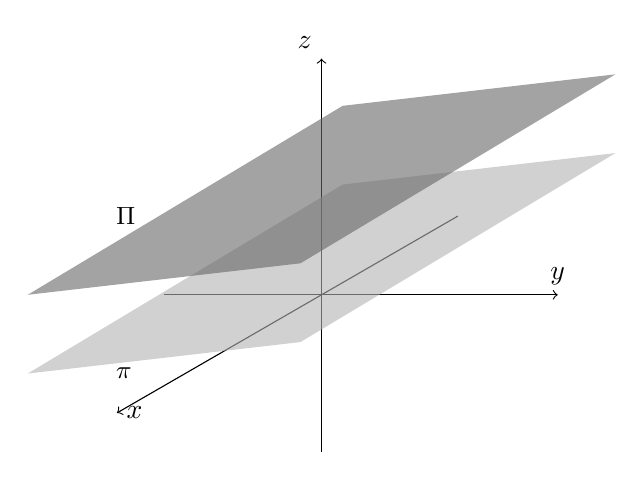
\begin{tikzpicture}[x={(-0.866cm,-0.5cm)}, y={(1cm,0cm)}, z={(0cm,1cm)},
      scale=1]
      % Ejes coordenados
      \draw[->] (-2,0,0) -- (3,0,0) node[right] {$x$};
      \draw[->] (0,-2,0) -- (0,3,0) node[above] {$y$};
      \draw[->] (0,0,-2) -- (0,0,3) node[above left] {$z$};

      % Primer plano: 2x + 3y - 5z + 2 = 0
      % Resolviendo para z: z = (-2x - 3y - 2)/-5
      \fill[opacity=0.6, black!30]
        (-2,-2,{(-2*(-2) - 3*(-2) - 2)/-5}) --
        (2,-2,{(-2*(2) - 3*(-2) - 2)/-5}) --
        (2,2,{(-2*(2) - 3*(2) - 2)/-5}) --
        (-2,2,{(-2*(-2) - 3*(2) - 2)/-5}) -- cycle;

      % Segundo plano: 2x + 3y - 5z + 7 = 0
      % Resolviendo para z: z = (-2x - 3y - 7)/-5
      \fill[opacity=0.6, black!60]
        (-2,-2,{(-2*(-2) - 3*(-2) - 7)/-5}) --
        (2,-2,{(-2*(2) - 3*(-2) - 7)/-5}) --
        (2,2,{(-2*(2) - 3*(2) - 7)/-5}) --
        (-2,2,{(-2*(-2) - 3*(2) - 7)/-5}) -- cycle;

      % Etiquetas de los planos
      \node at (2, -1, 2) [right] {\small $\Pi$};
      \node at (2, -1, 0) [right] {\small $\pi$};
    \end{tikzpicture}
    } % Fin del cambio de idioma
    \caption{Conjuntos disjuntos. Planos paralelos $\pi$ y $\Pi$}%
    \label{fig:planos-paralelos}
  \end{figure}

  % Quizás, le quite los colores. En realidad, no los necesito.
  \begin{figure}
    \centering
    \foreignlanguage{english}{% Cambio de idioma por error del paquete Babel
    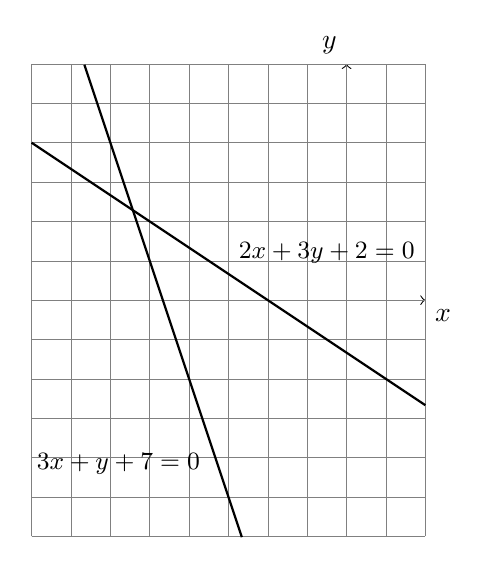
\begin{tikzpicture}[scale=1]
      % Ejes coordenados
      \draw[->] (-4,0) -- (1,0) node[below right] {$x$}; % Eje x
      \draw[->] (0,-3) -- (0,3) node[above left] {$y$};  % Eje y

      % Cuadrícula
      \draw[step=0.5,gray,very thin] (-4,-3) grid (1,3);

      % Primera recta: 2x + 3y + 2 = 0 -> y = -(2/3)x - 2/3
      \draw[thick]
        (-4, {-2/3*(-4) - 2/3}) -- (1, {-2/3*(1) - 2/3})
          node[pos=0.5, above right] {\small $2x + 3y + 2 = 0$};

      % Segunda recta: 3x + y + 7 = 0 -> y = -3x - 7
      \draw[thick]
        (-3.33, {-3*(-3.33) - 7}) -- (-1.33, {-3*(-1.33) - 7})
          node[pos=0.8, below left] {\small $3x + y + 7 = 0$};

      % % TODO Calcular el punto de corte y representarlo.
      % % Punto de intersección (-0.5, -1)
      % \filldraw[black] (-0.5,-1) circle (1.5pt); % Punto
      % \node[anchor=north west] at (-0.5,-1) {\small $(-0.5, -1)$};
    \end{tikzpicture}
    }
    \caption{Intersección de conjuntos: Rectas secantes}%
    \label{fig:interseccion_rectas}
  \end{figure}
\end{example}




\subsubsection{Propiedades distributivas}

Otra propiedad que se cumple es que la intersección es distributiva respecto
de la unión y la unión es distributiva respecto de la intersección. Es
decir, para tres conjuntos cualesquiera $A$, $B$ y $C$, se tiene

\begin{align*}
  A \cap (B \cup C) &= (A \cap B) \cup (A \cap C) \\
  A \cup (B \cap C) &= (A \cup B) \cap (A \cup C) \\
\end{align*}

Advierta que se cumplen las dos propiedades distributivas, mientras que con
los números se cumple únicamente la distributiva del producto respecto de la
suma.

\begin{exercise}
  Halle el conjunto de definición de la función real

  \[ f(x) = \frac{x^2 - 4}{x - 1} \]

  \noindent es decir, los valores de $x$ para los que existe $f(x)$.

  En principio, lo único que le impediría a la función tener valores de
  salida sería los que hagan que el discriminante de la raíz sea menor que 0
  y los que hagan que el divisor sea 0.

  Los valores de la variable $x$ para los que se tiene que el discriminante
  de la raíz es válido son, por tanto,

  \[ \left\{ x \in \rset \st \frac{x^2 - 4}{x - 1} \geq 0 \right\} \]

  \noindent Este conjunto es el mismo que

  \[ \{x \in \rset \st x^2 - 4 \leq 0 \ \text{y} \ x - 1 < 0\} \cup \{x \in
  \rset \st x^2 - 4 \geq 0 \ \text{y} \ x - 1 > 0\} \]

  \noindent ya que, para que una división sea mayor o igual a 0, tienen que
  ser el numerador y el denominador ambos positivos o ambos negativos, pero
  no con signos mezclados. Vamos a analizar ahora cada uno de esos conjuntos
  por separado.

  Por un lado, se tiene que

  \begin{align*}
    \{x \in \rset \st x^2 - 4 \leq 0 \ \text{y} \ x - 1 < 0\}
      &= \{x \in \rset \st x^2 - 4 \leq 0\}
      \cap \{x \in \rset \st x - 1 < 0\} \\
      &= [{-2}, 2] \cap ({-\infty}, 1) = [{-2}, 1)
  \end{align*}

  \noindent y, por el otro,

  \begin{align*}
    \{x \in \rset \st x^2 - 4 \geq 0 \ \text{y} \ x - 1 > 0\}
      &= \{x \in \rset \st x^2 - 4 \geq 0\}
      \cap \{x \in \rset \st x - 1 > 0\} \\
      &= [({-\infty}, {-2}] \cup [2, \infty)] \cap (1, \infty) \\
      &= [({-\infty}, {-2}] \cap (1, \infty)] \cup [[2, \infty)] \cap (1,
        \infty)] \\
      &= \emptyset \cup [2, \infty) = [2, \infty) \\
  \end{align*}

  \noindent Advierta que se ha usado una de las propiedades distributivas de
  la unión y la intersección. Además, se ha excluido el valor $x = 1$, pues
  ese valor hace 0 al denominador de la fracción.

  El resultado será, entonces,

  \[ [{-2}, 1) \cup [2, \infty) \]

  \noindent Puede comprobarlo en la figura~\ref{fig:dominio-partes}, que
  representa su gráfica.

  \begin{figure}
  \centering
    \foreignlanguage{english}{% Cambio de idioma por error del paquete Babel
    \begin{tikzpicture}[scale=1]
      % Ejes coordenados
      \draw[->] (-3,0) -- (5,0) node[below] {$x$};
      \draw[->] (0,-1) -- (0,5) node[left] {$y$};

      % Eje vertical en x=1 (asimptota vertical)
      \draw[dashed] (1,-1) -- (1,5);

      % Parte del dominio en el eje x
      \draw[very thick] (-2,0) -- (0.99,0); % Intervalo x <= -2
      \draw[very thick] (2,0) -- (5,0);  % Intervalo x >= 2

      % Etiquetas de los puntos en el eje x
      \filldraw (-2,0) circle (0.05cm) node[below] {$-2$};
      \filldraw (2,0) circle (0.05cm) node[below] {$2$};
      \draw (1,0) circle (0.05cm); % Punto abierto en x=1
      \node at (1, -0.2) [below, left] {$1$};

      % Graficar la función
      % f(x) = sqrt((x^2 - 4) / (x - 1))
      \draw[domain=-2:0.87, thick, samples=100]
        plot (\x, {sqrt(((\x)^2 - 4)/(\x-1))});
      \draw[domain=2:5, thick, samples=100]
        plot (\x, {sqrt(((\x)^2 - 4)/(\x-1))});

      % Etiqueta de la función
      \node at (-1.5,1.8) {$f(x)$};
    \end{tikzpicture}
    }
    \caption{Conjunto de definición de
      $f(x) = \sqrt{\frac{x^2 - 4}{x - 1}}$.}%
    \label{fig:dominio-partes}
  \end{figure}
\end{exercise}

Aunque la unión y la intersección están definidas únicamente para dos
conjuntos, resulta que las propiedades asociativas permiten definir la unión
y la intersección de tres o más conjuntos:

\begin{align*}
  A \cup B \cup C \quad &\text{y} \quad A \cup B \cup C \cup D \cup \cdots \\
  A \cap B \cap C \quad &\text{y} \quad A \cap B \cap C \cap D \cap \cdots \\
\end{align*}

\noindent Esto hace que en la notación se pueda prescindir del uso de
paréntesis a este respecto.





\subsection{Familia indexada de conjuntos}

Sea $I$ un conjunto que supondremos no vacío y al que llamaremos
\emph{conjunto de índices} de la familia. Supongamos que a cada $i \in I$,
es decir, a cada índice, le asociamos un conjunto $F_i$. La colección de
todos esos conjuntos $F_i$ se denomina \semph{familia de conjuntos} y se
denota por

$$ \mathcal{F} = \{F_i \st i \in I \} $$

\noindent Advierta que, aunque se diga \emph{familia}, en realidad no es más
que un conjunto: un conjunto de conjuntos. Lo califican de esta otra forma
para hacer una disttinción clara de los niveles de anidamiento. Se trata
también de una familia \emph{indexada} ya que cada conjunto se identifica
con un elemento del conjunto de índices. Concretamente, el conjunto de
índices suele estar formado por números naturales. Así, se tendría una
familia como, por ejemplo,

\[ F_1,\ F_2,\ F_3,\ \dots \]

Como es evidente, cuando todos los conjuntos $F_i$ son subconjuntos de un
mismo conjunto $U$, entonces $\mathcal{F}$ es un subconjunto del conjunto
$\powset(U)$. Recíprocamente, cualquier subconjunto $\mathcal{G}$ no vacío
de $\powset(U)$ será también una familia de conjuntos.

% TODO Quizás se pueda quitar lo de no vacío.

Los conceptos de unión e intersección se extienden a familias arbitrarias de
conjuntos, pues, tal y como hemos explicado, estas no dejan de ser conjuntos
al fin y al cabo.

Dada una familia de conjuntos $\mathcal{F} = \{F_i \st i \in I\}$ para un
conjunto de índices $I$, el conjunto unión de todos los conjuntos de la
familia $\mathcal{F}$ es el conjunto de los elementos que pertenecen al
menos a un $F_i$, siendo $i \in I$. Es decir:

$$ \bigcup_{i \in I} F_i = \{x \st \exists i \in I. \ x \in F_i\} $$

Si la familia viene dada por un subconjunto $\mathcal{G}$ no vacío de
$\powset(U)$, entonces la unión es

$$ \bigcup_{F \in \mathcal{G}} F = \{x \in U \st \exists F \in \mathcal{G}.
\ x \in F\} $$

Análogamente, el conjunto intersección de todos los conjuntos de la famnilia
$\mathcal{F}$ es el conjunto de los elementos comunes a todos los conjuntos
$F_i$, siendo $i \in I$. Es decir,

$$ \bigcap_{i \in I} F_i = \{x \st \forall i \in I. \ x \in F_i\} $$

Si la familia viene dada por un subconjunto $\mathcal{G}$ no vacío de
$\powset(U)$, entonces la intersección es

$$ \bigcap_{F \in \mathcal{G}} F = \{x \in U \st x \in F. \ \forall F \in
\mathcal{G}\} $$

\begin{exercise}[Intervalos Encajados]
  Dado $a \in \rset$, se considera la familia de intervalos cerrados

  \[ I_n = \left[ a - \frac{1}{n}, a + \frac{1}{n} \right] \subseteq \rset
  \]

  \noindent con $n \in \rset^*$. Demuestre que

  \begin{align*}
    \bigcap_{n \in \nset^*} I_n &= \{a\} \\
    \bigcup_{n \in \nset^*} I_n &= [a - 1, a + 1] \\
  \end{align*}

  Es evidente que $a \in \left[ a - 1/n, a + 1/n \right]$ para todo $n \in
  \nset^*$. Luego, $\{a\} \subseteq \bigcap_{n \in \nset^*} I_n$.

  Ahora, hay que demostrarlo en el otro sentido, es decir, que $\bigcap_{n
  \in \nset^*} I_n \subseteq \{a\}$. Lo haremos por contradicción.

  Supongamos que la inclusión $\bigcap_{n \in \nset^*} I_n \subseteq \{a\}$
  no es cierta. Entonces $\exists b \in \bigcap_{n \in \nset^*} I_n$ tal que
  $b \not\subseteq \{a\}$, o lo que es lo mismo, ya que $a$ es el único
  elemento de $\{a\}$, que $b \neq a$. Si tomamos $n_0 \in \nset^*$ tal que
  $\frac{1}{n_0} < |b - a|$, se tiene que $b \notin \left[ a - 1/n_0, a +
  1/n_0 \right]$, que está en contradicción con la suposición de que $b \in
  \bigcap_{n \in \nset^*} I_n \subseteq \{a\}$.

  La segunda igualdad que deseamos demostrar,

  \[ \bigcup_{n \in \nset^*} I_n = \left[a - 1, a + 1 \right] \]

  \noindent es evidente, pues la familia de intervalos satisface

  \[ [a - 1, a + 1] \supseteq \left[ a - \frac{1}{2}, a + \frac{1}{2}
  \right] \supseteq \left[ a - \frac{1}{3}, a + \frac{1}{3} \right]
  \supseteq \left[ a - \frac{1}{4}, a + \frac{1}{4} \right] \supseteq \cdots
  \]
\end{exercise}






\subsection{Diferencia y diferencia simétrica}

Dados dos conjuntos $A$ y $B$, el conjunto diferencia de $A$ y $B$, que se
escribe ``$A$ - $B$'' o ``$A \setminus B$'' y se lee ``$A$ menos $B$'', es
el conjunto de elementos que pertenecen a $A$ y no pertenecen a $B$. Es
decir,

$$ A \setminus B = \{x \st x \in A \ \text{y} \ x \notin B\} $$

En particular, si $A$ y $B$ son subconjuntos del conjunto $U$ y están
definidos por comprensión, como

\begin{align*}
  A &= \{x \in U \st P_x\} \\
  B &= \{x \in U \st Q_x\} \\
\end{align*}

\noindent entonces

$$ A \setminus B = \{x \in U \st P_x \land \neg Q_x\} $$



\subsubsection{Propiedades}

Se cumple que:

\begin{itemize}
  \item $A \setminus B = A \setminus (A \cap B)$.

  \item Si $A \subseteq U$ y $B \subseteq U$ y $\overline{B}$ es el
    complementario de $B$ en $U$, se cumple

    \begin{align*}
      U \setminus B = \overline{B} \\
      A \setminus B = A \cap \overline{B}
    \end{align*}
\end{itemize}

Esta última igualdad se puede considerar una definición alternativa de la
diferencia de conjuntos. De hecho, se usa más que la otra. La demostramos en
el ejercicio siguiente.

\begin{exercise}
  Demuéstrese que para todo par de conjuntos $A, B \in \powset(U)$, se
  cumple que $A \setminus B = A \cap \overline{B}$.

  Para ver la igualdad, comprobaremos las dos inclusiones:

  \[ A \setminus B \subseteq A \cap \overline{B}, \quad A \cap \overline{B}
  \subseteq A \setminus B \]

  Si $x \in A \setminus B$, entonces $x \in A$ y $x \notin B$, por
  definición de diferencia de conjuntos. Ahora bien, si $x \notin B$,
  entonces $x \in \overline{B}$, por definición de complementario de un
  conjunto. Luego, si $x \in A$ y $x \in \overline{B}$, entonces $x \in A
  \cap \overline{B}$, por definición de intersección de conjuntos, y, por lo
  tanto, $A \setminus B \subseteq A \cap \overline{B}$.

  Inversamente, si $x \in A \cap \overline{B}$  se tiene que $x \in A$ y $x
  \in \overline{B}$, por definición de intersección de conjuntos. Ahora
  bien, si $x \in \overline{B}$, entonces $x \notin B$, por defición de
  complementario de un conjunto. Luego, si $x \in A$ y $x \notin B$,
  entonces $x \in A \setminus B$, y, por tanto, $A \cap \overline{B}
  \subseteq A \setminus B$.
\end{exercise}

Dados dos conjuntos $A$ y $B$, el conjunto \semph{diferencia simétrica} de
$A$ y $B$, que se escribe $A \triangle B$, es el conjunto de elementos que
pertenecen solo a uno de los dos conjuntos $A$ y $B$. Son por tanto los
elementos de $A \cup B$ que no son elementos de $A \cap B$. Es decir,

\[ A \triangle B = (A \cup B) \setminus (A \cap B) \]

Se comprueba fácilmente que una definición al ternativa sería

\[ A \triangle B = (A \setminus B) \cup (B \setminus A) \]

\noindent o, lo que es lo mismo,

\[ A \triangle B = (A \cap \overline{B}) \cup (B \cap \overline{A}) \]

\noindent En consecuencia,

\[ A \triangle B = \{x \st x \in A \ \text{y} \ x \notin B\} \cup \{x \st x
\notin A \ \text{y} \ x \in B\} \]

En particular, si $A$ y $B$ son subconjuntos del conjunto $U$ y están
definidos por comprensión, como

\begin{align*}
  A = \{x \in U \st P_x\}
    & B = \{x \in U \st Q_x\}
\end{align*}

\noindent entonces,

\[ A \triangle B = \{x \in U \st (P_x \land \neg Q_x) \lor (\neg P_x \land
Q_x)\} \]

\begin{exercise}
  Demuestre que, dados dos conjuntos $A$ y $B$, se cumple que

  \[ A \setminus B = A \triangle (A \cap B) \]

  Para ver la igualdad, comprobaremos que se cumplen las dos inclusiones

  \begin{align*}
    A \setminus B &\subseteq A \triangle (A \cap B) \\
    A \setminus B &\supseteq A \triangle (A \cap B) \\
  \end{align*}

  Para la primera, sea un $x \in A \setminus B$ arbitrario. Entonces, $x \in
  A$ y $x \notin B$. En consecuencia, $x \notin A \cap B$. Luego $x \in A
  \setminus (A \cap B)$. Si nos fijamos en la definición de diferencia
  simétrica entre $A$ y $A \cap B$,

  \[ A \triangle (A \cap B) = [A \setminus (A \cap B)] \cup [B \setminus (A
  \cap B)] \]

  \noindent se dará, en particular, que $A \setminus (A \cap B) \subseteq A
  \triangle (A \cap B)$, con lo que $x \in A \triangle (A \cap B)$, y queda
  demostrada la primera parte.

  % TODO Está mal. Ponerme con esto.

  Para la segunda parte, de $x \in A \triangle (A \cap B)$ se cumple
  particularmente que $x \in A \setminus (A \cap B)$. De esto, se tiene que
  $x \in A$ y $x \notin A \cap B$, de lo que se deduce que $x \notin B$ pues
  en caso contrario, si fuera $x \in B$, resultaría que $x \in A \cap B$, en
  contradicción con $x \notin A \cap B$. Por tanto, $x \notin B$ y en
  consecuencia $x \in A \setminus B$.

  El segundo caso es imposible pues $A \cap B \subseteq A$.

  En definitiva, se cumple la inclusión $A \triangle (A \cap B) \subseteq A
  \setminus B$.
\end{exercise}








